\documentclass{kluwer}    % Specifies the document style.

\newdisplay{guess}{Conjecture}

% package provides \sout{} strikeout macro -- remove this before submission
\usepackage{ulem}

\usepackage{graphicx}

\newcommand{\arclabel}[1]{\ensuremath{\stackrel{#1}{\to}}}
\newcommand{\precision}[1]{\ensuremath{\textrm{Prec}\left(#1\right)}}
\newcommand{\recall}[1]{\ensuremath{\textrm{Recall}\left(#1\right)}}


\begin{document}
\begin{article}
\begin{opening}         
\title{Expected Dependency Pair Match:\\
Predicting {HTER} improvements with expected syntactic structure} 
\author{Jeremy G. \surname{Kahn}\email{jgk@u.washington.edu}}  
\institute{University of Washington}
\author{Matthew \surname{Snover}\email{snover@cs.umd.edu}}
\institute{University of Maryland}
\author{Mari \surname{Ostendorf}\email{ostendor@u.washington.edu}}  
\institute{University of Washington}
\runningauthor{Kahn, Snover \& Ostendorf}
\runningtitle{Expected Dependency Pair Match}
%s\date{May 10, 2009}

\begin{abstract}
Abstract to go here
\end{abstract}
\keywords{machine translation evaluation, syntax, dependency trees}

\end{opening}           

% override ulem 's default change of \emph{} -- remove before ship
\normalem
\section{Introduction}
\label{sec:intro}

\begin{itemize}
\item \sout{ evaluation [esp. automatic evaluation]}
\item \sout{popular current
  measures BLEU \cite{papineni02bleu}, TER}
\end{itemize}
Machine translation (MT) evaluation is a challenge for research
because the space of good translations is large, and two equally good
translations may appear to be quite different at first glance. 
%
The challenges of choosing among translations are compounded when this
evaluation is done automatically.
%
Human evaluation, however, is both time-consuming and difficult, so
research has turned increasingly towards automatic measures of
translation quality, usually by comparing the system translation to
one or more reference (human) translations.
%
Automatic measures of this kind (e.g.\ BLEU \cite{papineni02bleu}) not
only provide a well-defined evaluation standard but are also required
for training on error criteria, e.g.\ with minimum error rate training
\cite{och03mert}.

The most popular evaluation measures are currently BLEU (based on
$n$-gram precision) and the edit-distance measure Translation Edit
Rate (TER) \cite{snover06ter}.  Recent research has found that these
measures may not accurately track translation quality both empirically
\cite{charniak03syntaxlmmt} and theoretically
\cite{callisonburch06bleuproblems}.

\begin{itemize}
\item \sout{challenges - motivate search for better measures}
\item \sout{other extensions:}
  \begin{itemize}
  \item \sout{METEOR }
    \begin{itemize}
    \item \sout{stemming and synonym tables}
    \item \sout{tuned but not generally     tuneable}
    \end{itemize}
  \item \sout{TERp}
    \begin{itemize}
    \item \sout{development-set tuning by user}
    \item \sout{stemming and synonym tables}
    \item \sout{paraphrase tables}
    \end{itemize}
  \end{itemize}
\end{itemize}

These challenges have motivated a search for better measures that
incorporate additional language knowledge sources.  METEOR
\cite{banerjee05meteor}, for example, uses synonym tables and
morphological stemming to do progressively more-forgiving matching.
It can be tuned towards recall or precision, but is generally not
tuned by users.  TERp \cite{snover09terp} is an extension of the
previously-mentioned TER that also incorporates synonym sets, along
with automatically-derived paraphrase tables.  TERp is explicitly
intended to be tuned to a development set by users.

TO DO: DISCUSS TUNING'S VIRTUES, FLAWS


\begin{itemize}
\item \sout{prior work with (partial) syntactic locality:}
  \begin{itemize}
  \item \sout{Liu \& Gildea }
  \item \sout{Roark et al. Sparseval}
  \item \sout{Owczarzak et al. 2007}
  \end{itemize}
\end{itemize}

As an alternative to these synonym- and paraphrase-based approaches,
other metrics model syntactically-local (rather than string-local)
word-sequences. \cite{liu05syntaxformteval} compared tree-local
$n$-gram precision in various configurations of constituency and
dependency trees.  The dependent-based SParseval measure
\cite{roark06:sparseval}, originally designed as a parse-quality
metric for speech, is a similar approach, in that it is an F-measure
over a decomposition of reference and hypothesis trees.
\cite{owczarzak07labelleddepseval}'s \textbf{d} and \textbf{d\_var}
measures compare LFG-derived relational tuples from reference and
hypothesis translations and report substantial improvement in
correlation with human judgment relative to BLEU and TER.

These syntactically-oriented measures require a system for proposing
dependency structure over the reference and hypothesis
translations. Some \cite{liu05syntaxformteval,roark06:sparseval} use
PCFG parsers with deterministic head-finding, while others
\cite{owczarzak07labelleddepseval}extract the semantic dependency
relations from an LFG parser \cite{cahill04lfg}.
%
This work extends the dependency-scoring strategies of
\cite{roark06:sparseval,owczarzak07labelleddepseval} using a
widely-used and publically available PCFG parser and deterministic
head-finding rules.
 
\begin{itemize}
\item \sout{Evaluation of evaluation measures}
  \begin{itemize}
  \item \sout{correlation vs. human fluency/adequacy }
  \item \sout{correlation vs. human-in-the-loop measures (HTER)}
  \end{itemize}
\end{itemize}

We may evaluate automatic MT measures in a variety of ways. Some
\cite{banerjee05meteor,liu05syntaxformteval,owczarzak07labelleddepseval}
have evaluated their success by comparing the measure to human
judgments of fluency and adequacy.  In other work,
e.g. \cite{snover06ter}, measures are evaluated by comparison to
human-targeted TER (HTER), a distance to a human-revised reference
that uses wording closer to the MT system choices (keeping the
original meaning) that is intended to measure the post-editing work
required after translation.  In this paper, we explore both kinds of
evaluation.

TO DO: OVERVIEW OF THE REST OF THE PAPER



\section{Approach}
\label{sec:approach}

This work explores a family of dependency pair match (DPM) measures
that are composed of precision and recall combinations over various
decompositions of a syntactic dependency tree. These measures are
extensions of the dependency-pair F measures found in
\cite{roark06:sparseval,owczarzak07labelleddepseval}.  Rather than
comparing string sequences, as BLEU does with its $n$-gram precision,
this approach defers to a parser for an indication of the relevant
words that indicate more about its meaning --- in these
implementations, the head on which that word depends.  Each sentence
(both reference and hypothesis) is converted to a labeled syntactic
dependency tree and then relations from each tree are extracted and
compared.

A member of this family is defined by several parameters.  The first
of these parameters is the nature of the decomposition of the
dependency tree structure.  A \emph{decomposition list} is the list of
ways in which the tree is reduced to a bag of tree-local
tuples. Figure~\ref{fig:decompexample}
\begin{figure}
  \centering
  \begin{tabular}{rcc}
    & \textbf{Reference} & \textbf{Hypothesis} \\
    \textbf{dependency tree}
    & 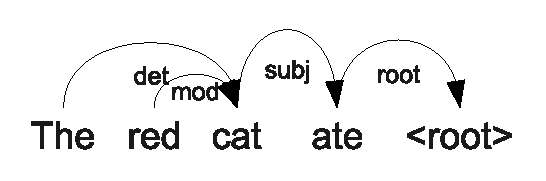
\includegraphics[scale=0.6]{dpm-example-ref.eps} & 
    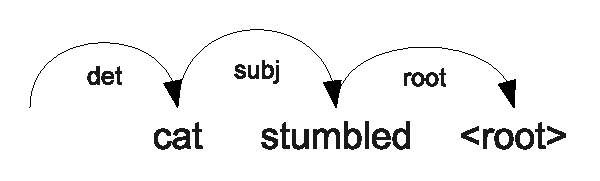
\includegraphics[scale=0.6]{dpm-example-hyp.eps}\\
    \textbf{$dlh$ list} &
    \begin{tabular}{@{$\langle$}c@{,~}c@{,~}c@{$\rangle$}}
      the & \arclabel{\texttt{det}}  &  cat \\
      red & \arclabel{\texttt{mod}}  &  cat \\
      cat & \arclabel{\texttt{subj}} &  ate \\
      ate & \arclabel{\texttt{root}} &  $<$root$>$ \\
    \end{tabular} & 
    \begin{tabular}{@{$\langle$}c@{,~}c@{,~}c@{$\rangle$}}
      the &      \arclabel{\texttt{det}}  &  cat \\
      cat &      \arclabel{\texttt{subj}} &  stumbled \\
      stumbled & \arclabel{\texttt{root}} &  $<$root$>$ \\
    \end{tabular}\\
  \end{tabular}\\
  Precision$_{dlh}$ is $\frac{1}{3}$ and Recall$_{dlh}$ is
  $\frac{1}{4}$, so $F[dlh] = \frac{2}{7}$
  \caption{Example hypothesis and reference dependency trees and the $dlh$ decomposition of each.}
  \label{fig:decompexample}
\end{figure}
illustrates the \emph{dependency-link-head} decomposition of the
dependency tree into a list of $\langle d, l, h \rangle$ tuples.  Some
members of the DPM family may apply more than one decomposition; other
good examples are the $dl$ decomposition, which generates a bag of
dependent word with outbound links, and the $lh$ decomposition, which
generates a bag of inbound link labels, with the head word for each
included.

It is worth noting here that the $dlh$ and $lh$ decompositions (but
not the $dl$ decomposition) ``overweight'' the headwords, in that
there are $n$ elements in the resulting bag, but if a word has no
dependents it is found in the resulting bag exactly one time (in the
$dlh$ case) or not at all (in the $lh$ case).  Conversely,
syntactically ``key'' words, that are directly modified by many other
words in the tree, are included multiple times in the decomposition
(once for each inbound link).  We argue that this overcounting is a
virtue; the syntactic structure indicates which words are more
important to translate correctly.

We may not completely trust the parser's best parse.  The parser
itself, if we use a probabilistic parser, can provide an $n$-best
parse list forest for the translation reference and translation
hypothesis. We use the probability statistics of the forest to compute
expected counts for each decomposition. Though this approach yields
partial counts, standard comparisons like precision and recall are
still valid.

When multiple decomposition types used together, we may combine these
subscores in a variety of ways.  We may compute precision and recall
subscores for each decomposition separately, or, since the results of
each decomposition are of different types entirely, we may compute
them as members of one large bag for an even simpler F score.  These
two approaches are equivalent when only one decomposition type is
included.  For simplicity in presentation, we use the following
notation, where $dl$ and $lh$ represent the two kinds of
decompositions described above and $\mu_h$ represents a harmonic mean:
\begin{eqnarray}
  \label{eq:fprmeans}
  F[dl,lh] & = &
  \mu_h \left( \precision{dl \cup lh},
    \recall{dl \cup lh} \right) \\
  \mu_{PR}[dl,lh]  & = & \mu_h \left( \precision{dl},
    \recall{dl}, \precision{lh}, \recall{lh} \right)    
\end{eqnarray}
Dependency-based SParseval and Owczarzak \textit{et al.}'s
\cite*{owczarzak07labelleddepseval} \textbf{d} approach, then, may
each be understood as $F[dlh]$, while the latter's \textbf{d\_var}
method may be understood as something close to $F[dl,lh]$.




Outline of big idea here.

\begin{itemize}
\item comparison of various bags of components of parse tree
  [ Figure describing Sparseval-ish variant ]

  Like sparseval: basic unit is labeled dependency pair

  Note: inbound links \& full pairs "overweight" head words; this is
  a good thing.

  [ figure demonstrating F-measure over d+l+h decomposition of toy
  trees ]
    
\item Tree features may be extracted from a 1-best tree, or from an
  n-best tree list 

\item elements may be combined in various ways: single-bag F, combination of p,r
  measures (evenly, on analogy with BLEU)... or we might weight
  different combinations

\end{itemize}
\section{Experimental paradigm}
\label{sec:paradigm}

Section explains space of measures to explore, mean-normalization

\begin{itemize}
\item Listing possible component valences
  \begin{itemize}
  \item dependent + labeled link + head 
  \item outbound only (dependent +
    label)
  \item inbound only (label + head)
  \item word-word (skipping label)
  \end{itemize}
  \begin{itemize}
  \item 1-grams
  \item 2-grams
  \item \ldots{}
  \end{itemize}
  
    
\item Tree features may be extracted from a 1-best tree, or from an
  n-best tree list 

  \begin{itemize}
  \item  counts are an expectation over the forest
  \item n parameter: how many trees in the forest
  \item gamma parameter for flattening overconfident parse hyps
  \end{itemize}
  note intentional similarities to Owczarzak paper


\item Components in the basic DPM measures combined in various ways:

  \begin{itemize}
  \item combination of precision, recall scores for different
    components (on analogy with BLEU combination), naive assumption:
    all weighted equally

  \item simple F over items of all valences (naive assumption: all
    weighted equally)
  \end{itemize}
\item Tuneable weights:
  \begin{itemize}
  \item recall that TERp has tuneable system over small number of parameters
    \begin{itemize}
    \item insertion weight
    \item deletion weight
    \item substitution weight
    \item synonym weight (motivated with WordNet)
    \end{itemize}
  \item learn weights for separate precision, recall for various
    components
  \end{itemize}
  
\item Implementation
  \begin{itemize}
  \item Charniak parser
  \item n=1..50
  \item head-finding, with some modifications
  \item label-construction
  \end{itemize}

\begin{itemize}
\item \sout{one challenge of metric-evaluation: underlying doc difficulty }
  \begin{itemize}
  \item \sout{describe mean-subtraction}
  \end{itemize}
\end{itemize}
When considering a candidate measure $m$, reporting correlations of
$m$ with absolute HTER scores can conflate $m$'s power in identifying
which of two candidate translations is better with $m$'s (and HTER)'s
ability to distinguish which of two source documents is more difficult
to translate. To avoid this conflation, we consider the mean-removed
$m$ and HTER scores; this lowers the correlations but ensures that the
reported correlations are among differences in the translations rather
than among differences in the underlying document.

\end{itemize}

\section{Correlation with human judgments of fluency \& adequacy}
\label{sec:faexpts}
Corpus: LDC Multiple Translation Chinese corpus 3\&4 treat each
segment and each judgment as independent data point

\begin{itemize}
\item EXPT

  using n=1 parse for DPM variants

\begin{verbatim}
   metric      r
  --------   -----
  F[dl;lh]   0.226
  BLEU4      0.218  # +1 smoothing
  F[dlh]     0.185
  TER       -0.173
\end{verbatim}

  point: using partial-labeling (dl,lh) much better than full
  link. Also, using Charniak parser as labeler seems to work, LFG not
  necessary

\item EXPT 

  combining precision, recall naively vs. combining items

\begin{verbatim}
  F(1g,2g,dl,lh)        0.237
  prmeans(1g,2g,dl,lh)  0.217

  F(dl,lh)              0.226
  prmeans(dl,lh)        0.208
\end{verbatim}

  point: combining individual items naively (before computing
  precision and recall) seems better than naively combining precisions
  and recalls (too many chances for zeroes?)

\item EXPT
  expanding n, gamma=0

\begin{verbatim}
  F[1g,2g,dl,lh],n=50   0.239
    ...          n=1    0.237
  F[dl,lh],n=50         0.234
    ...    n=1          0.226
\end{verbatim}
  point: larger n $\to$ better r
  (holds for other comparisons too, but these are good examples)

\item  EXPT

  setting gamma

  Tuning experiments finds that gamma of 0.25 is slightly better
  (especially when using F[dl,lh]) than gammas of other values in
  range 0-1 (these values probably not significant)

\end{itemize}

\section{Correlations with HTER}
\label{sec:hter1}
  Corpus
    Gale translation corpus 2.5; 3 sites, 2 source languages, 4 genres each

  prediction:
    Mean-subtracted HTER per-document

  base measure EDPM: F[1g,2g,dl,lh],n=50,gamma=0.25

  [EXPT]
\begin{verbatim}
            Ar     Zh    All
   TER     0.51   0.32  0.44
   BLEU_4 -0.42  -0.33 -0.37
   EDPM   -0.60* -0.39 -0.50*
\end{verbatim}
  point: base EDPM does better on all docs, and on Arabic. difference
  is not quite significant at the p=0.05 on the Chinese documents

  Note 1: also tried pairwise deltas per-document, with similar
  results, as presented in the MetricsMATR competition submission.

  Note 2: when using per-segment mean-subtracted, r values are smaller
  and *Arabic* was the language where EDPM did not perform best.

\begin{verbatim}
               Ar     Zh     All
      TER     0.38*  0.04   0.19
      BLEU_4 -0.10  -0.16  -0.14
      EDPM   -0.31  -0.19* -0.24*
\end{verbatim}

  (Go into details of per-genre differences here? or leave out, for
  space reasons? -- leave out, I'd say)

\section{Weight-tuning to combine syntax and other knowledge sources}
\label{sec:hter2}

TERp optimizer [Matt, a brief description here]

TERp comes with a variety of features (described earlier)

include optionally new features

Corpus: GALE 2.5 data, again documents randomly split into two groups,
evenly split across language and genre

tuning target: weighted correlation with mean-removed segment HTER

[we use weighted correlation to avoid emphasis on short segments
(which hurts document-level and system-level utility) ]

Select features from set:

\begin{description}
\item[E]: features from EDPM, specifically, P,R for inbound, outbound,
  full-links, and unlabeled links  (8 features)
\item[T]: features from basic TERp
  (inserts, deletes, substitutions, shifts)  (7 features)
\item[P]: features from TERp paraphraser
  (4 features)
\item[N]: precision and recall for 1-grams, 2-grams
\item[B]: brevity/prolixity (2 features: one for longer-than-ref, one for
  shorter-than-ref)
\end{description}

tune weights on one set, test on the other (and vice versa).
reporting average r between the two.

\begin{verbatim}
   == Tuned For Weighted Mean Removed Pearson
     - Examining WGT_MEAN_RM_SEG_PEAR ==
            Average
      Cond   Test  
     ---------------
      ETPB   0.4096
      ETP    0.4038
      TPB    0.4010
      TP     0.3946
      TPNB   0.3940
      TPN    0.3891
      ETB    0.3871
      ET     0.3827
      TB     0.3815
      ETNB   0.3814
      ETN    0.3804
      T      0.3758
      TNB    0.3708
      TN     0.3680
      E      0.3287
      EB     0.3267
      ENB    0.3149
      NB     0.3058
      EN     0.2973
      N      0.2636
      B      0.1638
\end{verbatim}
(maybe don't report all these numbers!)
  
point: E+T $>$ T, E+TB $>$ TB, E+TP $>$ TP; information is available in
syntax that is not captured in the other measures.

point: syntax is *not* just an expensive way to get at n-grams;
N-grams are not the same -- TP $>$ TP+N, but TP $<$ TP+E

\section{Conclusion}
\label{sec:conclusion}
expected dependency pair matching gets at something new

troubling area: speed of analysis -- current implementation requires
running a complete n-best parser

possible use: as a late-pass evaluation, to identify how systems
perform overall

future work:  explore ways to get at syntactic information without
the expense of a full parser:
\begin{itemize}
\item this work moves from an LFG parser (Owczarzak) to the
  substantially simpler and more robust Charniak system - keep going
  and look at simpler partial-parsing approaches (forests?)
\item conversely: how important is it that the parses be of
  high-quality?
\end{itemize}





\appendix

[don't think we want an appendix]


\acknowledgements

[grant numbers for the DARPA/GALE grants here]

% The endnotes section will be placed here.  But I don't think we have any

% \theendnotes

\bibliographystyle{klunamed}
\bibliography{edpm-paper}

\end{article}
\end{document}
